\documentclass{article}
\usepackage{color}
\usepackage[usenames,dvipsnames]{xcolor}
\usepackage{listings}	
\usepackage{enumerate}
\usepackage{layouts}
\usepackage{times}
\usepackage{natbib}
\usepackage{notoccite}
\usepackage{todonotes}
\usepackage{alltt}
\usepackage{url}
\usepackage{amsmath}
\usepackage{amsfonts}
\usepackage{amsthm}
\usepackage{xspace}
\usepackage{tikz}
\usepackage[dvipsnames]{xcolor}
\usepackage{subcaption}

\usepackage{fancyvrb}

\theoremstyle{definition}
\newtheorem{definition}{Definition}[section]
\newcommand{\triple}[1]{\ensuremath{\langle #1 \rangle}}
\newcommand{\pair}[1]{\ensuremath{\left(#1\right)}}
\newcommand{\graph}[1]{\ensuremath{\mathcal{#1}}}
\newcommand{\graphset}[1]{\ensuremath{\mathbb{#1}}}

\newcommand{\sergey}[1]{\textcolor{magenta}{\marginpar{\sc Sergey} #1}}
\newcommand{\matthias}[1]{\textcolor{blue}{\marginpar{\sc Matthias} #1}}
\newcommand{\Qone}{$\boldsymbol{Q_1}$\xspace}
\newcommand{\Qtwo}{$\boldsymbol{Q_2}$\xspace}
\newcommand{\Qthree}{$\boldsymbol{Q_3}$\xspace}

\lstdefinestyle{model}{
  mathescape,
  columns=fullflexible,
  numbers=none,
  frame=single,
  escapechar=@
}

% redefine \VerbatimInput
\RecustomVerbatimCommand{\VerbatimInput}{VerbatimInput}%
{fontsize=\footnotesize,
   %
  frame=lines,  % top and bottom rule only
  framesep=2em, % separation between frame and text
  rulecolor=\color{Gray},
      %
  label=\fbox{\color{Black}proB encoding},
  labelposition=topline,
        %
% commandchars=\|\(\), % escape character and argument delimiters for
                              % commands within the verbatim
% commentchar=*        % comment character
}

\author{Authors}
\title{Note on KR and Graph Mining}
\begin{document}
\maketitle

\section{Introduction}
\sergey{feel free to rephrase and correct me here, that's an early attempt to set up a story}
Frequent Pattern Mining, one of the ''super-problems`` in Data Mining, has received significant attention over the last years \citep{pattern_mining_book}. Especially useful in applications has turned out to be structured mining such as graph mining, where one is looking for sub-structures that often occur in the data, e.g., a graph that is a subgraph of many graphs in the dataset. Recently, there is a line of work towards declarative pattern mining \citep{tias_declarative_pattern_mining} and today we look into declarative structured pattern mining that just started receiving attention in both data mining and knowledge representation communities \citep{cp_sequence_mining,ilp_graph_mining}. A main motivation for this approach is that it can accommodate multiple version of a problem under the same roof (such as different forms of homomorphism checks in graph mining) .


\matthias{We still need to mention the different types of homomorphism/isomorphisms.}There are two most common ``matching'' notions in structured pattern mining: in ILP literature they are $\theta$-subsumption and OI-subsumption and in Data Mining literature they are known as homomorphism and subgraph isomorphism \citep{jan_ramon}. \sergey{I am not sure where to put it exactly but not in the introduction}


Our main goal is to investigate the problem of graph mining from the knowledge representation perspective and more concretely we are going to look in the following questions:
\begin{itemize}
  \item[\Qone:]   What is the logical model of the frequent graph mining problem?
  \item[\Qtwo:]   How this model can be implemented in the existing logic programming languages?
  \item[\Qthree:] Do all necessary concepts and primitives already present in the existing logic programming languages?
\end{itemize}

\sergey{we need a smooth transition here or should we just start a new section like ``formalization''?}

%\subsection{Problem definition}
\begin{definition}
\label{def:GM1}
Given a pair $\triple{\graphset{E}_{+},\graphset{E}_{-}}$ consisting of a set of \emph{positive} and \emph{negative} examples of \emph{labeled graphs}, respectively,
\emph{Graph mining} is the problem of finding one \emph{connected labeled graph} $\graph{P}$, called a \emph{pattern},
that is \emph{homomorphic} with at least $N_{+}$ positive, while homomorphic with at most $N_{-}$ negative examples.
\end{definition}

\begin{definition}
A graph $\graph{G} = \triple{V,E,l}$, where $V$ is the set of vertices, $E$ the set of edges and $l$ the labeling function, is \emph{connected} iff for each pair of vertices $v$ and $v'$ in $V$, there exists an edge $\pair{v,v'} \in E$ or there exists a sequence $v \ldots v_{1} \ldots v_{n} \ldots v'$ such that there exist edges $\pair{v,v_{1}}$, $\pair{v_{i},v_{i+1}}$ and $\pair{v_{n},v'} \in E$.
\end{definition}


\begin{definition}
A graph homomorphism $f$ from labeled graph $\graph{G} = (V,E,l)$ to $\graph{G}' = (V',E',l')$, where $V$ is the set of vertices, $E$ the set of edges and $l$ the labeling function, is an injective mapping f : $V \rightarrow V'$ from vertices of $\graph{G}$ to vertices of $\graph{G'}$ s.t. 
\begin{itemize}
\item $\forall u,v \in V, \pair{u,v} \in E \implies \pair{f(u),f(v)} \in E'$ (the mapping preserves edges), and 
\item $\forall v \in V : l(v) = l(f(v))$ (the mapping respects labelings).
\end{itemize}
If there exists such a graph homomorphism between graphs $\graph{G}$ and $\graph{G'}$ we say $\graph{G}$ is \emph{homomorphic} with $\graph{G'}$.
\end{definition}

\begin{figure}[h]
  \centering
  \begin{subfigure}[b]{0.3\textwidth}
    \centering
    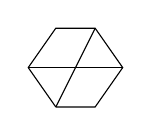
\begin{tikzpicture}[scale=.5]
      \draw (1,1) -- (2,1) -- (2.7,2) -- (2,3) -- (1,3) -- (0.3,2) -- (1,1);
      \draw (1,1) -- (2,3);
      \draw (2.7,2) -- (0.3,2);
    \end{tikzpicture}
    \caption{Positive Example\label{fig:pos}}
  \end{subfigure}
  ~
  \begin{subfigure}[b]{0.3\textwidth}
    \centering
    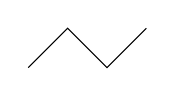
\begin{tikzpicture}[scale=.5]
      \coordinate (1) at (0,0);
      \coordinate (2) at (1,1);
      \coordinate (3) at (2,0);
      \coordinate (4) at (3,1);
      \draw (1) -- (2) -- (3) -- (4);
    \end{tikzpicture}
    \caption{Negative Example\label{fig:neg}}
  \end{subfigure}
  ~
  \begin{subfigure}[b]{0.3\textwidth}
    {
      \setcounter{subfigure}{0}
      \renewcommand\thesubfigure{\Roman{subfigure}}
      \centering
      \begin{subfigure}[b]{0.45\textwidth}
        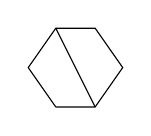
\begin{tikzpicture}[scale=.5]
          \draw (1,1) -- (2,1) -- (2.7,2) -- (2,3) -- (1,3) -- (0.3,2) -- (1,1);
          \draw (2,1) -- (1,3);
        \end{tikzpicture}
        \caption{Valid\label{fig:correctcandidate}}
      \end{subfigure}
      ~
      \begin{subfigure}[b]{0.45\textwidth}
        \begin{tikzpicture}[scale=.5]
          \draw (1,2) -- (2,3) -- (3,3);
        \end{tikzpicture}
        \caption{Invalid\label{fig:incorrectcandidate}}
      \end{subfigure}
    }
    \caption{Pattern Candidates\label{fig:candidates}}
  \end{subfigure}
  \caption{Example 1:\label{fig:ex1}}
\end{figure}

%    \begin{tikzpicture}[scale=.5]
%        \coordinate (1) at (0,0);
%        \coordinate (2) at (1,1);
%        \coordinate (3) at (2,0);
%        \coordinate (4) at (3,1);
%        \draw (1) --
%              (2) --
%              (3) --
%              (4);
%    \end{tikzpicture}, ...

Take, for example, the problem set shown in Figure~\ref{fig:ex1}.
There is one positive example (Fig~\ref{fig:pos}), and one negative example (Fig~\ref{fig:neg})
We assume all nodes have the same label.
Figure \ref{fig:candidates} shows a valid and an invalid pattern.
Requiring at least one homomorphism with a positive example, and allowing no homomorphisms with negative examples (i.e. problem parameters $N_{+}=1$ and $N_{-}=0$), only Figure \ref{fig:correctcandidate} represents a valid pattern.
It is clear that there exists a mapping from each node from the valid pattern to a node of the positive example, while no such mapping exists for the negative example.
Looking at Figure \ref{fig:correctcandidate}, this graph is clearly homomorphic with both the positive as well as the negative example. Therefore, it is not a pattern.

\subsection{Canonical patterns}
To extend on this graph mining task described above, we can look for multiple patterns, instead of just one.
In this case, one can impose restrictions on the different patterns that are found.
For example, it stands to reason that one wants only \emph{canonical} solutions, meaning that no two patterns found are \emph{isomorphic}.

\begin{definition}
\label{def:isomorphism}
A graph isomorphism $f$ between two labeled graph $\graph{G} = \triple{V,E,l}$ and $\graph{G'} = \triple{V',E',l'}$ is a \emph{one-to-one} mapping $V \rightarrow V'$ 
such that $f$ represents a homomorphism from $\graph{G}$ to $\graph{G'}$,
and its inverse $f^{-1}$ represents a homomorphism from $\graph{G'}$ to $\graph{G}$.
If there exists such a graph isomorphism between $\graph{G}$ and $\graph{G'}$ we say $\graph{G}$ and $\graph{G'}$ are \emph{isomorphic}.
\end{definition}

We now want to define the concept of a canonization and the related concept of a canonical graph. 
%Having defined the concept of a homomorphism, we want to define the concept of a \emph{canonical} graph.
To define this concept, we need to consider a multitude of graphs $\graph{G}$, each of which consists of a set of vertices $V$, an edge relation $E$ and a labeling function $l$. 
As the vertices themselves have no distinctive property, it is possible, and even beneficial to reuse the same, sufficiently large set of vertices $V$ for all example graphs as well as the mined patterns.

\begin{definition}
\label{def:canonicalForm}
Let $\graphset{G}$ be a set of graphs over a sufficiently large set of vertices $V$, closed under isomorphism.
A function $c$ for which $\forall \graph{G,H} \in \graphset{G} : \graph{G} \simeq \graph{H} \iff c(\graph{G}) = c(\graph{H})$ and $\forall \graph{G} \in \graphset{G} : \graph{G} \simeq c(\graph{G})$ hold, is called a \emph{canonization}.
The graph $c(\graph{G})$ is called the \emph{canonical form} w.r.t $c$, and is denoted by $\mathit{canon}(\graph{G})$.
\end{definition}

\begin{figure}[h]
  \centering
  \begin{subfigure}[b]{0.45\textwidth}
    \centering
    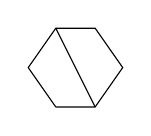
\begin{tikzpicture}[scale=.5]
      \draw (1,1) -- (2,1) -- (2.7,2) -- (2,3) -- (1,3) -- (0.3,2) -- (1,1);
      \draw (2,1) -- (1,3);
    \end{tikzpicture}
    \caption{First candidate pattern\label{fig:iso1}}
  \end{subfigure}
  ~
  \begin{subfigure}[b]{0.45\textwidth}
    \centering
    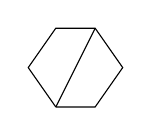
\begin{tikzpicture}[scale=.5]
      \draw (1,1) -- (2,1) -- (2.7,2) -- (2,3) -- (1,3) -- (0.3,2) -- (1,1);
      \draw (1,1) -- (2,3);
    \end{tikzpicture}
    \caption{Second candidate pattern\label{fig:iso2}}
  \end{subfigure}
  \caption{Possible patterns\label{fig:isomorphism}}
\end{figure}

Given the graph mining problem as specified in Figure~\ref{fig:ex1}, we have already established that Figure~\ref{fig:iso1} is a valid pattern.
When we try to mine a second pattern, we might suggest a pattern as shown in Figure~\ref{fig:iso2}.
A quick check, however, will show that there is a one-to-one mapping $f$ such that both $f$ as well as its inverse $f^{-1}$ preserve edges.
As a result, the first candidate pattern and the second are isomorphic.
By Definition~\ref{def:canonicalForm} only one of these two patterns can be the canonical form, and therefore only one of these two candidate patterns should be accepted as a valid pattern.

\subsection{Rewording}
%Given the mathematical definition of the graph mining problem above, w
We want to study how this can be expressed in the logics underlying the IDP~\cite{} and the ProB~\cite{} system.
First, we will reword the earlier definition~\textbf{Def.}~\ref{def:GM1} into an equivalent formal definition that uses logical sentences and language constructs available in general logics.
In doing this, it becomes evident that the graph mining problem has fundamental underlying characteristics that result in a higher order definition and specification.

%An attempt to model the Graph Mining problem in both IDP as well as ProB makes it clear
%that neither language allows us to express the problem to its full extent.
%We now try to link the shortcomings of each language to the expressiveness of the underlying logic on which they are built.

%First we introduce a new definition of the graph mining problem, equivalent to \textbf{Def.}~\ref{def:GM1}.
As mentioned above, the vertices in the graph mining problem have no distinctive property, and can be reused between different example graphs and patterns.
Therefore, we will assume one shared, sufficiently large set of vertices $V$ and represent example graphs over these vertices $V$ directly as a triple $\triple{Edge, Label, Class}$, consisting of an edge relation between $V$ and a labeling function over $V$, as well as a classification (positive/negative).

\begin{definition} \textbf{Graph Mining (redefined)}
\label{def:gm2}
Given a sufficiently large set of vertices $V$, and a set $\graphset{G}$ of graphs over this vertex set $V$, represented by $\triple{E, l, c}$ triples
where $E$ and $l$ represent the edge relation and labeling function over $V$ respectively,
%which consist of an edge relation, 
we look for a 
%(set $\graphset{P}$ of) \todo{cleanly extend this definition to multiple graphs, or separate the single and multiple pattern case again}
graph represented by tuple $\triple{E_{\graph{P}}, l_{\graph{P}}}$ such that:
%for at least $N_{+}$ of the triples $\triple{ E, l, C}$ with $C=Pos$, and for at most $N_{-}$ of such triples with $C=Neg$, there exists a function $f$ s.t. $\forall u,v \in V, \pair{u,v} \in E_{p} \implies \pair{f(u),f(v)} \in E$ and $\forall v \in V : l_{p}(v) = l(f(v))$.

\todo{draft: possible different wording}
\begin{itemize}
\item $\#\Big\lbrace \triple{E,l,pos} \in \graphset{G} \; | \; \exists f : \text{f is an homomorphism from \graph{P} to \triple{E,l,pos}} \Big\rbrace \geq N_{+}$

\item $\#\Big\lbrace \triple{E,l,neg} \in \graphset{G} \; | \; \exists f : \text{f is an homomorphism from \graph{P} to \triple{E,l,neg}} \Big\rbrace \leq N_{-}$
\end{itemize}
\end{definition}

\begin{definition} \textbf{Canonical Patterns}

\end{definition}

As evidenced from the definitions above, graphs are the main concept in the graph mining problem, and, as a triple $\triple{V,l,c}$ are inherent \emph{higher order objects}.
A set of graphs, such as the argument of the cardinality operator above or the set of example graphs $\graphset{G}$, is equivalent to a set of triples.
The most straightforward representation of such a set would therefore be a ternary predicate.
As the domains of this predicate range over predicates and functions, this predicate would be a higher order predicate.

It is a very natural KR representation to consider each graph as a \emph{coherent} ensemble of its own components: all characteristics (edges, labeling \ldots) of a graph are represented by separate entities or concepts, which are grouped together for each graph $\graph{G}$ in the triple that describes it. We refer to this as the \emph{local coherence} of the graph representation.
Not only is this a very natural KR representation, this representation also makes it very explicit that all example graphs are \emph{independent}, and that the search for a homomorphism between pattern and example graph is independent as well.

It becomes clear that we want to reason about graphs as locally coherent objects in our logical models as well.
However, the higher order representations needed to reason about graphs and sets of graphs as \emph{coherent} objects in our models are not yet fully supported by the logics of IDP and ProB.
In the following section we discuss how we can deal with this.

%When reasoning about graphs, we see \emph{each graph} as a \emph{coherent} ensemble of its own components: 
%all characteristics (edges, labeling \ldots) of a graph are represented by separate entities or concepts, which are grouped together for each graph $\graph{G}$ in the triple that describes it.
%We refer to this as the \emph{local coherence} of the graph representation.
%As graphs are the main concepts we talk about in the graph mining problem, keeping this concept together leads to a natural KR representation.
%Furthermore, this locally coherent representation makes it very explicit that all example graphs are \emph{independent}, and that the search for a homomorphism between pattern and example graph is independent as well.
%A good solver can then discover this independence and leverage it to achieve better performance.

%A set of graphs, such as the argument of the cardinality operator above or the set of example graphs $\graphset{G}$, is equivalent to a set of triples.
%The most straightforward representation of such a set would therefore be a ternary predicate.
%As the domains of this predicate range over predicates and functions, this predicate would be a higher order predicate.

%These higher order representations for graphs and sets of graphs are not yet fully supported by the logics of IDP and ProB.
%In the following section we discuss how we deal with them.
%\todo{Illustrate local coherence with table}

\section{Related Work}
There is a number of research directions related to our work. We group them by what they have in common with our work and contrast the difference with each group.

\paragraph{Declarative Pattern Mining} There has been a lot of work on declarative pattern mining for unstructured data focused on: \textit{itemset mining} in the context of constraint programming \citep{tias_original,mining_cp_extra,tias_declarative_pattern_mining}, as well as in ASP \citep{asp_itemset} and SAT \citep{itemset_sat}, and \textit{tiling} in the context of ASP \citep{relational_decomposition} and of CP \citep{ranked_tiling}. 

Recently people started looking at the structured declarative pattern mining such as \textit{sequence mining} in CP \citep{cp_sequence_mining} and ASP \citep{rennes_asp_sequences}, and \textit{graph mining} in IDP \citep{ilp_graph_mining}. \sergey{I hope by this time IDP is very well explained and introduced, so I can just leave it as ``it is''} The main focus of these works is on the encoding techniques that allows one to encode model using existing language concepts and primitives, i.e., on the coding and execution but not on the model and language itself. From the KR point view, the latter work on graph mining is of a preliminary character, since it does not provide a deep knowledge representation analysis of the model with respect to the mismatch between higher order logical model and the executed model. Neither the most interesting practical case of discriminative mining was not investigated in detail, nor any comparison between ASP, IDP and ProB was provided. \sergey{Should it be phrased less harsh here?}

\sergey{to do: CP(graph) \citep{cp_graph}, reference to Siegfried survey \citep{subtree_overview} -- many ways to define matching ``subtree'' for example, Anton's + Sigfried's mining under theta subsumption \citep{theta_subsumption} -- means we need different matching, \citep{declarative_structured_language} -- need to explain how this can be used to create a generic solver without much overhead}

\section{Modellings}
\subsection{IDP}
\subsubsection{Existential Second Order}
The IDP language can express problems that consist of a set of symbols, called the vocabulary $V$, and a theory, called $T$, that uses symbols from this vocabulary.
The symbols in the vocabulary can be propositions, but they can also represent predicates and functions.
These last two types of symbols make the vocabulary, in general, a \emph{second order} object: it is an object that itself \emph{contains} not only propositional symbols, but also first order symbols.
For example, vocabulary V in Listing \ref{lst:vocabularyExample} is a second order vocabulary as it contains the first order symbol \lstinline{Edge/2}.

The theory $T$ is restricted to a \emph{first order} theory, extended with arithmetic, aggregates, and inductive definitions.
An example of such a theory is given in Listing \ref{lst:vocabularyExample}.

Our inference of choice in the graph mining problem is model expansion; we search for an interpretation $I$ of symbols in the vocabulary $V$ such that this interpretation $I$ satisfies the theory $T$.
This corresponds to the implicit \emph{existential quantification} of all symbols in the vocabulary, both the first order as well as the second order symbols.

In conclusion, we say IDP can express model expansion for \emph{Existential Second Order} problems.

\begin{lstlisting}[mathescape,basicstyle=\fontfamily{lmvtt}\selectfont,caption=\ldots, label=lst:vocabularyExample]
Vocabulary V{
    type Node
    p
    q
    Edge(Node, Node)
}
Theory T : V {
    $\forall$n : $\exists$n2[Node] Edge(n,n2) | Edge(n2,n).
    p => q.
}
Structure S : V{
    Node = {1,2,3}
    p
}
\end{lstlisting}
\begin{lstlisting}
Structure Result:V{
    p
    q
    Edge = {1,1;1,2;2,3}
}
\end{lstlisting}


%problems in which there is an existentially quantified, generally second order, vocabulary of symbols and a first order theory with symbols from that vocabulary.
\paragraph{Issue 1}
First, we must represent the set of example graphs, as specified in \textbf{Def.}~\ref{def:gm2}. 
This definition uses a higher order predicate, as shown in \textbf{Listing}~\ref{lst:HOPred}. 
It represents a single graph as a tuple of predicates and functions, visualised in \textbf{fig.}~\ref{fig:LocalCoherence} as the solid shape.
It is clear that this representation is highly locally coherent, and preserves the independence of graph characteristics.
However, as we are restricted to \emph{Existential} Second Order, we cannot express this higher order predicate.

One possible solution is to replicate for each graph the different characteristic predicates and functions, as well as the knowledge (theory) about them, as shown in
in \textbf{Listing}~\ref{lst:multiglobal} and visualised as the dashed shape in \textbf{Fig.}~\ref{fig:LocalCoherence}.
This way of representing the information about graphs is shown in Listing~\ref{lst:multiglobal}.
It is clear that this solution is undesirable due to the way it scales and the editing needed with growing problem instances.
It retains the local coherence and independence of graph characteristics when it comes to data representation, but prohibits the abstraction (generalization) of knowledge about these properties, as evidenced by our obligation to duplicate the theory for each graph.

%GraphInst(E:Node$\times$Node,Lb
\begin{lstlisting}[mathescape,caption=Higher order predicate modelling the set $\graphset{G}$ of Def~\ref{def:gm2}.,label=lst:HOPred]
GraphInst({(1,2),(2,1)},{1$\mapsto$a,2$\mapsto$b},pos).
GraphInst({(1,3),(2,1)},{1$\mapsto$c,2$\mapsto$b,3$\mapsto$a},neg).
\end{lstlisting}
\begin{minipage}[t]{0.5\textwidth}
\begin{lstlisting}[mathescape,caption=Multiple global relations,label=lst:multiglobal]
E1(1,2). lb1(1)=a.
E1(2,1). lb1(2)=b.
E2(1,3). lb2(1)=c.
E2(2,1). lb2(2)=b.
         lb2(3)=a.
\end{lstlisting}
\end{minipage}
\begin{minipage}[t]{0.5\textwidth}
\begin{lstlisting}[mathescape,caption=Indexed global relation,label=lst:indexedglobal]
E(g1,1,2). lb(g1,1)=a.
E(g1,2,1). lb(g1,2)=b.
E(g2,1,3). lb(g2,1)=c.
E(g2,2,1). lb(g2,2)=b.
           lb(g2,3)=a.
\end{lstlisting}
\end{minipage}




A more workable solution is to represent each characteristic property, such as the edge relation, by a single general relation for all graphs, as shown in \textbf{Listing}~\ref{lst:indexedglobal} and by the dotted shape in \textbf{Fig.}~\ref{fig:LocalCoherence}.
This relation behaves the way it should for a specific graph instance based on an additional argument serving as an identifier for the graph of interest.
%This gives rise to a set $G$ of \emph{graph identifiers}, one for each example graph.
This general relation now corresponds to the \emph{disjoint} or \emph{tagged union} of the graphs' relations, where the tags are drawn from a set $G$ consisting of graph identifiers.
It is clear that this representation forces us to give up the local coherence of graph characteristics that was present in \textbf{Def.}~\ref{def:gm2}: 
%Nu kunnen we kijken wat deze truuk doet met onze mogelijkheid om de abstraction van de theory uit te drukken. Normaal mwillen we dit zo schrijven. Hoewel we nu de generalisatie kunnen uitdrukken, verplicht de restrictie tot existentieel s..o ons om de homomorphic mapping functies te tot een globale property te promoveren, hoewel we feitelijk niet geinteresseerd zijn in de concrete mappings. om om te gaan met de afhankelijkheid van deze functies op de spec. vb grafen moeten we... die nu erg lijkt op skolemisation. theory

%Using this trick however, does not influence our ability to 

But can we now express the abstraction (generalization) of knowledge about these properties, such as the positive homomorphic property?
%to separate the constraint describing the positive homomorphic property, and the coint on its number of occurrences.
%This, from a KR point of view, 
%Furthermore, the restriction to ESO requires us 
%As an example, we illustrate this trick by showing on the expression of the positive homomorphic property, where it greatly resembles Skolemization.
As evidenced in \textbf{Def.}~\ref{def:gm2}, normally one would express the positive homomorphic property by quantifying (counting) over all graphs, requiring the existence of a function with the correct properties.
Using this trick, does not influence our ability to express this restriction: Instead of quantifying over the graphs themselves, we can now quantify over the set $G$ of graph identifiers.

\begin{figure}[h]
\centering
\begin{tabular}{l |l l l}
         & $E$ & $l$      & $c$ \\
\hline
$\graph{G}_{1}$  & $E_{1}$ & $l_{1}$ & pos\\
$\graph{G}_{2}$  & $E_{2}$ & $l_{2}$ & pos\\
  \vdots & \vdots  & \vdots  & \vdots\\
$\graph{G}_{n}$  & $E_{n}$ & $l_{n}$ & pos\\
\end{tabular}
\caption{Local coherence\label{fig:LocalCoherence}}
\end{figure}

\begin{tikzpicture}[overlay]
  \draw [dotted, rounded corners](4.8,4) -- (4.8,1.5) -- 
  (5.3,1.5) -- (5.3,4) -- cycle;
  \draw [rounded corners] (3.9,2.66)--(7.18,2.66) --
  (7.18,3.1) -- (3.9,3.08) -- cycle;
  (3.south east) -- (3.south west);
  \draw [dashed, rounded corners] (5.05,2.85) circle (3mm);
\end{tikzpicture}

%These three different ways of representing graphs are summarized in Fig~\ref{fig:LocalCoherence}.

\paragraph{Issue 2}
%Having solved\matthias{circumvented?} our first issue, 
Next, we would like to express the homomorphic property, as shown in Listing \ref{QuantifyOutsideVocabulary}.
\begin{lstlisting}[mathescape, caption=Quantifying over functions outside the vocabulary, label=QuantifyOutsideVocabulary,basicstyle=\fontfamily{lmvtt}\selectfont]
#{$\forall g$ : $\exists$ f : $\ldots$ }
\end{lstlisting}
However, the restriction to ESO forbids us to quantify over first-order entities such as functions outside of the vocabulary.
Thus, we are required to promote the homomorphic mapping functions to a global property in the vocabulary, even though we are only interested in the existence of a mapping, and not in a concrete valid mapping itself.
We prevent the same explosion of mapping functions as with the graph characteristics above, using the same method as above (which in this case corresponds to Skolemization):
We introduce a general function \verb|f| that represents all homomorphisms, and make its dependency on a specific example graph explicit using an additional argument:
\verb|partial f(graphId, t_var):node|.
%As it is impossible
%We introduce a general function \verb|f| that represents the homomorphisms, and make its dependency on a specific goal graph explicit using an additional argument:
In Second Order Logic, this dependency would follow directly from the order of the separate quantifications.

We can now use this \verb|partial f| anywhere we would use the regular homomorphic function for a specific graph by fixing the chosen example graph.
Note that this encoding also requires us to make this function \verb|f| partial, as the Graph Mining problem does not require the solution to be homomorphic with \emph{all} example graphs.
%\todo{Of course, other (even uglier) schemes exist to encode this. Should we mention this?}


\paragraph{Issue 3} Much in the same way, limiting ourselves to existential second order prohibits us from expressing the negative constraint on homomorphism (No more than $N_{-}$ negative examples are homomorphic) in the same model.
In fact, the negative constraint asserts a property for all candidate homomorphic functions, which would lead to \emph{universal} quantification.
Therefore, our only recourse is to encode its dual positive constraint and require it to fail when queried.\matthias{Find a convincing but small example}
\matthias{The moment to introduce the asp saturation technique}

\subsubsection{Inductive Definitions}
Beyond the Existential Second Order restriction, the IDP language is also extended with inductive definitions. These definitions, evaluated under the well-founded semantics, allows the derivation of negative knowledge that otherwise would be underivable. \matthias{Find a convincing but small example}
\reversemarginpar
\todo{A section about inductive definitions, and their use. (Being able to derive negative knowledge)}

\subsection{Faithful encoding}
\begin{alltt}
  //Homomorphism/2 is a higher-order predicate:
  //Edge1 and Edge2 are predicates themselves.
  homomorphism(<Edge1,Label1>, <Edge2,Label2>) 
  \(\iff \exists\) f: (\(\forall\) x, y : x \(\neq\) y \(\Rightarrow\) f(x) \(\neq\) f(y)) \(\wedge\)
  (\(\forall\)x, y : Edge1(x, y) \(\implies\) Edge2(f (x), f (y))) \(\wedge\)
  (\(\forall\) x : Label1(x) = Label2(f(x)))


  \textbraceleft
  reachable(x,y,Edge) \(\leftarrow\) Edge(x,y) \(\lor\) Edge(y,x).
  reachable(x,y,Edge) \(\leftarrow \exists\) : reachable(x,z,Edge) \(\wedge\) reachable(z,y,Edge).
  \textbraceright

  isomorph(<Edge1,Label1>,<Edge2,Label2>) \(\iff\)
      \big(\(\exists\)f : (\(\forall\) x,y:Edge1(x,y) \(\iff\) Edge2(f(x),f(y))) \(\wedge\)
      (\(\forall\) x : Label1(x) = Label2(f(x))) \(\wedge\)
      (\(\forall\)x,y:x\(\neq\)y\(\implies\)f(x)\(\neq\)f(y))\big).

  //\(\forall\)Pat represents quantification over a predicate Pat/2. 
  //A pattern is represented by its Edge relation. 
  \(\forall\)P : pattern(P) \(\implies\) #\textbraceleft Pos : positive(Pos) \(\wedge\) homomorphism(P, Pos) \textbraceright \(\geq\) \(N{+}\).
  \(\forall\)P : pattern(P) \(\implies\) #\textbraceleft Neg : negative(Neg) \(\wedge\) homomorphism(P, Neg) \textbraceright \(\leq\) \(N_\).
  \(\forall\)P,P2 :pattern(P)\(\wedge\)pattern(P2)\(\wedge\)P\(\neq\)P2 \(\iff\) \(\neg\)isomorph(P,P2).

\end{alltt}
\reversemarginpar
\todo{Tekstuele uitleg hierbij}

\subsection{ProB}

\section{Related Work}
\sergey{to be expanded}


\section{Feature Comparison}

\subsection{IDP} 

\textbf{Pro:}
\begin{itemize}
  \item can model inductive definitions
  \item allows core formulation in a high-level language (NP)
  \item handles aggregates
  \item has support for variety of constraints
\end{itemize}
\textbf{Cons:}
\begin{itemize}
  \item cannot handle negative case $\textit{NP}^\textit{NP}$ complexity
  \item cannot model subgraph isomorphism independence
  \item cannot handle dominance, i.e., when one model is preferred over another 
\end{itemize}

\paragraph{ASP}
Let us describe a way to encode the problem into ASP. Conceptually we need to handle three constraints: matching of positive examples, not matching of negative examples and canonicity (that only not isomorphic graphs are produced).

\lstset{basicstyle=\footnotesize\ttfamily,breaklines=true}
\begin{lstlisting}[caption=ASP positive matching, style=model]
positive_match(G) | not_positive_match(G) :- positive(G).

1 { map(G,X,V) : node(G,V) } 1 :- positive(G), invar(X).

:- positive_match(G), map(G,X,V1), map(G,Y,V2), t_edge(X,Y), 
not edge(G,V1,V2), invar(X), invar(Y).

positive_count(N) :- N = #count{G:positive_match(G)}.

:- positive_count(N), N < 2.
\end{lstlisting}

\begin{lstlisting}[caption=ASP negative matching, style=model]
%Saturated Representation

%negative constraints to check not matching negative graphs

map(G,X,v1) | map(G,X,v2) | map(G,X,v3) | map(G,X,v4) :- invar(X), negative(G).

map(G,X,V) :- saturated(G), t_node(X), node(G,V).

saturated(G) :- t_edge(X,Y), map(G,X,V1), map(G,Y,V2), not edge(G,V1,V2), negative(G), invar(X), invar(Y).
saturated(G) :- map(G,X,V),  map(G,Y,V), X != Y, invar(X), invar(Y). // we cannot map two different template nodes to the same 

negative_match(G) :- not saturated(G), negative(G).

negative_count(N) :- N = #count{G:negative_match(G)}.

:- negative_count(N), N > 1.

\end{lstlisting}

\begin{lstlisting}[caption=Canonicity template-based check, style=model]
iso(X,x1) | iso(X,x2) | iso(X,x3) | iso(X,x4) :- invar(X).

candidate_var(X) :- iso(_,X).

%not iso!
iso_saturated :- invar(X1), invar(X2), iso(X1,V1), iso(X2,V2),     t_edge(V1,V2), not t_edge(X1,X2). 
iso_saturated :- invar(X1), invar(X2), iso(X1,V1), iso(X2,V2), not t_edge(V1,V2),     t_edge(X1,X2).

iso(X,V) :- invar(X), t_node(V), iso_saturated.

d1(X) :-     invar(X), not candidate_var(X). 
d2(X) :- not invar(X),     candidate_var(X).

not_equal :- d1(X). % check that in fact candidate is different from the pattern itself
not_equal :- d2(X). % check that in fact candidate is different from the pattern itself

iso_saturated :- not not_equal. % should not be completely equal

min_d1(N) :- N = #min{ X: d1(X) }, not iso_saturated.
min_d2(N) :- N = #min{ X: d2(X) }, not iso_saturated.

iso_saturated :- min_d1(N1), min_d2(N2), N1 > N2.
\end{lstlisting}

\begin{lstlisting}[caption=Auxilary predicates -- probably should be moved to appendix, style=model]
%selects subpattern

t_path(X,Y) :- t_edge(X,Y), invar(X), invar(Y).
t_path(X,Y) :- t_edge(X,Z), t_path(Z,Y), invar(X).

:- invar(X), invar(Y), not t_path(X,Y).

0 { invar(X) } 1 :- t_node(X).
% auxilary constraints


edge(G,Y,X) :- edge(G,X,Y).
t_edge(Y,X) :- t_edge(X,Y).
node(G,Y)   :- edge(G,Y,_).
t_node(X)   :- t_edge(X,_).
\end{lstlisting}

\begin{lstlisting}[caption=Canonicity previous solution isomorphism check, style=model]
iso(s1,X,x1) | iso(s1,X,x2) :- invar(X).
iso(s2,X,x2) | iso(s2,X,x3) :- invar(X).

candidate_var(G,X) :- iso(G,_,X).

iso_saturated(G) :- invar(X1), invar(X2), iso(G,X1,V1), iso(G,X2,V2),     t_edge(V1,V2), not t_edge(X1,X2). 
iso_saturated(G) :- invar(X1), invar(X2), iso(G,X1,V1), iso(G,X2,V2), not t_edge(V1,V2),     t_edge(X1,X2). 
iso_saturatea(G) :- not equal(G), iso(G,_,_). 

iso(G,X,V) :- invar(X), t_node(V), iso_saturated(G).

:- not iso_saturated(G), iso(G,_,_).

d1(G,X) :-     invar(X), not candidate_var(G,X), iso(G,_,_).
d2(G,X) :- not invar(X),     candidate_var(G,X).

not_equal(G) :- d1(G,X). % check that in fact candidate is different from the pattern itself
not_equal(G) :- d2(G,X). % check that in fact candidate is different from the pattern itself

equal(G) :- not not_equal(G), iso(G,_,_).
\end{lstlisting}


\subsection{proB}
\textbf{Pro:}
\begin{itemize}
  \item can model negative case
  \item can model subgraph isomorphism independence
\end{itemize}
\textbf{Cons:}
\begin{itemize}
  \item cannot handle inductive definitions
  \item cannot handle different types of aggregates (? needs to be checked again)
\end{itemize}

the rest of constraints? 

\section{Code in ProB and IDP}

\VerbatimInput{original_prob_files/PositiveAndNegative.mch}
\pagebreak

\VerbatimInput[label=IDP encoding]{IDPencoding/core_constraints.idp}

\bibliography{references}
\bibliographystyle{abbrvnat}
\setcitestyle{authoryear,open={(},close={)}}

\end{document}
